\batchmode
\documentclass{article}


% Notes to potential editors:
% 1. Please don't change the line wrapping.  Exactly one sentence per line!
% 2. Update "date" and "version" below with each update
% 3. Notation :
%       Program names and other text to be typed by user or returned by the computer in {\tt }
%       Variables or arguments in {\em } or in $<$ $>$

\usepackage{fullpage}
\usepackage{graphicx}
\usepackage{fancyvrb}
\usepackage{url}
\usepackage{color}
\usepackage[T1]{fontenc}
\definecolor{darkblue}{rgb}{0,0.2,0.4}
\usepackage[colorlinks,linkcolor=darkblue,citecolor=blue,urlcolor=blue,pdftitle={fourfit user's manual},pdfauthor={Roger Cappallo}]{hyperref}
\usepackage[titletoc]{appendix}
\usepackage[parfill]{parskip}

\begin{document}

\newcommand{\Oa}[1]{\hspace{-12pt}\makebox[12pt]{$\star$}#1}
\newcommand{\Da}[1]{\hspace{-12pt}\makebox[12pt]{$\times$}#1}
\newcommand{\bfit}[1]{{\textrm{\textit{\textmd{#1}}}}}


\begin{center}

\vspace{5pt}

{\LARGE fourfit user's manual}

\vspace{5pt}

{\Large Version 1.0}


\vspace{10pt}

{\it Roger Cappallo}

\vspace{5pt}

MIT Haystack Observatory

\vspace{5pt}
\today

\end{center}

\tableofcontents

\section{Introduction}
This manual is intended to be useful for a varied audience, which will
include both users and developers. Hopefully it is organized enough
so that any specific user can find the information they need, although
of course the ultimate arbiter is the source code, which should be
consulted for further detail.

\subsection{Why fringe-fit?}
One might reasonably ask why fringe-fitting is even necessary, given that
the data have already been "correlated". The reason is that correlation
is done with a very specific model, which incorporates information about
source coordinates, station coordinates, epoch, frequency sequence, polar
motion, earth rotation, clock-settings, etc. Many of these parameters
contain significant errors, which will manifest themselves as non-zero
residual delay and phase, varying in time. It is the task of fringe-fitting
to remove as much of this residual signal as possible by estimating corrections
to the intermediate quantities of group delay and delay rate.

Once corrections to delay and rate are estimated, they can then be recombined
with the delay and rate predicted by the model, in order to yield a "total"
observable. This total is relatively insensitive to errors in the original
model. For example, if we define $O$ as the observed (true) value and $C$ 
as the computed model value, then the residual data value is $O-C$, and we 
have the relation $O = C + (O-C)$. Small changes to $C$ are canceled out by
compensating changes in $O-C$, at least over the region where changes
remain linear.

\subsection{Correlator windows}
Not only is it desirable to keep the model as close to reality as possible,
in order to stay within the linear region, but there are also some natural
limitations inherent in the correlation process, which cause a finite range
of possible residual values around the model. For example, a lag correlator
has a finite number of lags, and there is a maximum lag between the two 
datastreams, typically of order of 1 or 2 $\mu$s. The models must agree
with reality to this level, or the correlated signal will fall outside
the range of correlation. An FX correlator has similar limitations. If the
delay rate residual is too large, then the fringe phase may wrap around
a half or a full turn per accumulation period, causing loss of fringes or
weakened fringes, respectively. The natural multiband delay window is set 
by the spacing of the frequencies of the channels. It is the inverse of the
GCD of the all of the channel frequency differences.

For all three windows the natural window can be further restricted in
the post-processing. This is done in order to speed up the fringe search,
or possibly to restrict the range of a parameter based upon externally-
supplied information.


\section{History}
In the late 70Õs Alan Rogers developed a program called FRNGE derived from the original VLBI2 fringe-fitting program. It was written in fortran and designed to be efficient on an HP-21MX (later renamed to HP-1000) minicomputer. This computer had only 32K x 16 bit words, and was extremely slow by 21st century standards. Just performing the fringe-fitting on small scans in several minutes time was a real tour de force.

As both hardware and software technology improved it became apparent that FRNGE would need to be rewritten, and so fourfit was created by Colin Lonsdale, Roger Cappallo, and Cris Niell in the early 90Õs. The basic algorithms were adopted directly from FRNGE, while the I/O, control architecture, and plotting were heavily modified. The programming language was changed from fortran to C.


\section{Program control}
\subsection{\textbf command line}
The \textit{fourfit} command line has a number of options, which are
detailed in Appendix \ref{app:commandlineoptions}. 
Depending on the chosen options, each execution of \textit{fourfit}
could process any combination of:
\begin{itemize}
\item one or more scans
\item one or more baselines
\item one or more frequency bands
\item one or more polarization products
\end{itemize}
The most commonly used options include -t to invoke test mode,
which doesn't create any output files, -b to specify a particular
baseline to process, -p to pop up a fringe plot on the screen,
and -c to specify a control file name.


\subsection{\textbf control file}
Control files are the principal means by which \textit{fourfit} is usually controlled.
There is normally one control file created per experiment, with finer control
of processing provided within an experiment by using optional selectors,
such as specifying a time range or particular scans,
within the control file. Control file information can in turn come through
three different routes, in the order they are read:
\begin{enumerate}
\item there is the capability (not normally used) of having
a default control file. If it exists, it is accessed by
an environment variable called \$DEF\_CONTROL. It might prove useful
if the program defaults need to be changed on a regular basis.
\item a control file that may be referenced
through the -c option of the \textit{fourfit} command line
\item a convenience feature that allows immediate use of control file commands
on the run line (see \textbf{set} below)
\end{enumerate}
If the same parameters are set in more than one location it is the last
setting that is used.

\subsection{\textbf{set} mechanism}
As explained above, the final control file input to the program
is anything on the command line following \textbf{set}, if that is present.
Since it comes last, the information - if it matches the selector
criteria - overwrites any corresponding earlier information. For example,
the experiment control file might specify the singleband delay range over
which to search, but one could override it by appending 
\textbf{set sb\_win 0.56 0.56}, which would force it to use the value of 
0.56 $\mu$secs. This mechanism provides a convenient way to see the
effect of quick changes to parameters, since it avoids having to edit
the control file.


\section{Program output}
At the end of each fringe fit data are written to type 2
files within the current fileset, unless the program is
run in test mode with -t. These files contain all of the
information relevant to the fringe fit, and become the
input for subsequent astronomic or geodetic processing.
Optionally, a fringe plot may be popped up in a window,
or perhaps printed, in order to facilitate data quality
analysis.


\section{Architecture}
\subsection{control files}
Internally, the control files are implemented as a chained list of
structures, which are created and appended in the order that the control
file information
is encountered by the program (i.e. default control file first, then the
main control file, then any \textbf{set} commands.) The control block structures
each have four selectors, which control whether or not a particular
block will be applied to data. The selectors are (baseline, source, frequency
group, and time range), with wildcard matching allowed. A fifth 
"pseudo-selector" is a single-character station code such as K. It is expanded
internally into two identical parameter blocks, one matching baseline K? and the
next matching ?K. In addition to the selectors there are many parameters
that can be applied to the data, such as filtering parameters, calibration
corrections, or search ranges.

The control file is parsed by a finite-state machine, which can at times
react to errant input files so as to produce syntax error messages 
that are a little hard to interpret. The offending input line is always
printed, though, to help the user zero in on the problem.

The principal routines used in the control file parsing are:
\begin{itemize}
\item create\_fsm -- sets up a structure with the finite-state-machine information
containing the semantics of the control file commands
\item parse\_cmdline -- parses the command line options
\item parse\_control\_file -- high level routine that reads the control file, sets up
the fsm, uses lex, and invokes the parser
\item lex -- does a lexical analysis, changing keywords into tokenized information
\item parser -- does the heavy lifting of applying the fsm semantics to the tokenized
output of lex, in order to create c\_blocks
\end{itemize}

\subsection{fringe search}
The fringe search in \textit{fourfit} is a two-stage process:

\begin{enumerate}
\item Search over a large 3-dimensional grid of (singleband delay,
multiband delay, delay-rate) to find the approximate location of
the maximum of the delay resolution function.

\item Form a 5x5x5 cube of correlation amplitude 
values centered on the location found in the grid search, and
perform a 3 dimensional interpolation to find the peak value.
Note: this section describes the \textit{simultaneous} interpolation,
not the now-deprecated \textit{iterative} interpolation.
\end{enumerate}

\subsubsection{grid search}
A search is made through a large number of grid points
in a 3-dimensional volume with axes of singleband delay,
multiband delay, and delay-rate. The function being maximized
is the coherent sum of all of the correlator output
complex visibility points over frequency and time. The grid points are
evenly spaced, which allows the search to be done efficiently via
FFT's. For example, along the delay-rate axis the transform
of the complex phasors converts from a function of time
to a function of fringe frequency. The best fit can be found
by inspecting the fringe frequency values to find the maximum.
Similar conjugate searches in the delay domains are done: the
cross-power spectral points within the channels determine the
singleband delay peak, and the phases across the different
channels determine the multiband delay peak.
\subsubsection{interpolation}
Once the location of the maximum grid point is known, then an
interpolation step refines the values in the neighborhood of
that (singleband delay, multiband delay, delay-rate) triple.
In the interpolation step a direct summation of the complex visibility
values is performed, by rotating the data by a complex phase 
factor (see next section). This factor incorporates the effect of the offsets
along each of the three axes of a 5x5x5 cube, which is centered
on the values (sbd, mbd, dr) from the grid search.
After the cube is formed, the 3 coordinates of the maximum
of the visibility magnitude is found via iterative application
of a simultaneous 3-D interpolation. The iteration step is implemented
by searching for the maximum of an interpolated 11x11x11 cube
of visibility magnitudes. Each iteration has a 11x11x11 cube that
is a factor of 5 smaller, until all 3 coordinate spacings are
less than 0.0001 of the original 5x5x5 spacing.
\subsubsection{complex phase factor}
In the interpolation of the best-fit (mbd, sbd, dr) values and also
in the plotting of the data as fit by the program, there is
a complex rotation applied to the data. This factor has
the form $e^{-i 2 \pi \theta}$, where $\theta$ is given by
\begin{equation}
        \theta = f \Delta t \dot{\tau} + (f - f_{ref}) \tau_{mb} + b \tau_{sb}
\end{equation}
where:

\begin{tabular}{ll}
    $f$         & frequency of a data point \\
    $f_{ref}$   & reference frequency \\
    $\Delta t$  & offset in time of data from ref. time \\
    $\dot{\tau}$ & residual delay rate \\
    $\tau_{mb}$ & residual multiband delay \\
    $\tau_{sb}$ & residual singleband delay \\
    $b$         & (0.25, 0, -0.25) for (usb, dsb, lsb) data \\
\end{tabular}
\subsubsection{program structure}
The overall program structure can be seen in the calling
graphs of Appendix \ref{app:callinggraphs}.


\section{Algorithms}
\subsection {Ionosphere}

In the S/X geodetic system independent group delay estimates
are made for X-band and S-band, and a linear combination of these
delays,
$\tau_g=1.081 \tau_x - 0.081 \tau_s$,
is used to give a group delay measurement that is largely
free of ionospheric effects. One drawback of this system is that
both the S and X band obervations have to have a high enough 
signal-to-noise ratio so that a good detection can be made in each band.
In constrast,
the VGOS system is designed to work with very short scans, in which
the individual bands may not provide a reliable detection, and
in which all 4 bands need to be combined coherently in a fit. Since
this fit also spans a wide frequency range, it is necessary to
fit and remove the differential ionosphere from the group delay
estimate.

The phase contribution in radians due to the ionosphere, 
$\Delta \phi$, is 

\begin{equation}
        \Delta \phi = -8.448 x 10^9 \Delta TEC / f
\end{equation}
%
where f is the observing frequency in Hz, and 
$\Delta TEC \equiv TEC_a - TEC_b$ is the differential TEC
for baseline \textit{ab} in TEC units 
(1 TEC unit = $10^{16}$ elec $/ m^2$). 
\textit{NOTE! This definition of the sense of the differential
quantity as reference minus remote is (unfortunately) the opposite
of the standard used throughout the rest of fourfit.}
Since phase is only measured modulo $2\pi$, there is a non-linear
dependence of phase upon the $\Delta$TEC parameter in the
model, which restricts the manner in which a fit might
be performed.

\begin{figure}[tb]
  \centering
  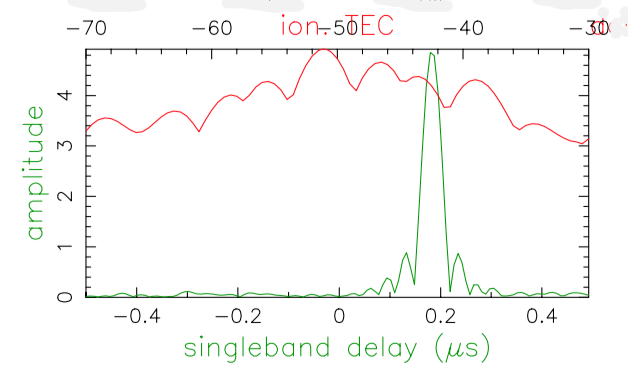
\includegraphics[width=.5\linewidth]{./ionosphere2.png}
  \caption{Ionospheric fit - correlation amplitude as a function of differential TEC
in TEC units (red curve). A complete fringe
fit at multiple points for trial values of the ionospheric
differential TEC is performed, and the code finds
the interpolated maximum.}
  \label{fig:ionosphere}
\end{figure}


The original algorithm used was that a range of coarse values 
were specified, the maximum within the range was found, then a second pass fine search
was done around the maximum. 
Recently the \textit{fourfit} code has been modified in a modest way,
in order to increase
the ionosphere search to be 3 level - (coarse, medium, fine). The
intent is to allow efficient searches over a wider range of $\Delta$TEC.

It is currently parameterized to allow a flexible coarse search, though
it is recommended that the user employs a 4 TEC unit spacing 
of the grid points over a wide range of $\Delta$TEC values. The fringe fit 
in Figure \ref{fig:ionosphere} used:
\begin{itemize}
    \item{coarse}: 11 points from (-70, -30)
    \item{medium}: 11 points with 2 unit spacing = +/- 10 units about the coarse peak
    \item{fine}: 11 points with 0.4 unit spacing = +/- 2 units about the medium peak
    \item{final}: parabolic interpolation of three fine points around the fine point peak
\end{itemize}

The medium and fine spacings are automatically generated; as before,
the user only supplies the coarse range and npts.
Though the efficiency of this algorithm could possibly
be improved, it has proven a very robust mechanism for finding the maximum value.

\subsubsection {Smoothing}

There is an option, invoked by ion\_smooth true (default: false)
in the fourfit control file. If invoked, the
code will do a 2-pass (as opposed to 3-pass) search
of TEC space, looking for the amplitude maximum. The
coarse spacing is determined by ion\_win and ion\_npts,
as before:

coarse\_step = (ion\_win[1] - ion\_win[0]) / (ion.npts - 1)

The smoothing code takes the grid points from the coarse
search and performs a convolutional smoothing, using
a half-cycle of a cosine function as the smoothing kernel.
It then finds the maximum of the smoothed, interpolated
new points. Execution of this step takes negligible time.

A final fine search is then done about the smoothed
maximum, of double width (of the non-smoothed fine search
- i.e. 24 pts) at 0.4 TEC unit spacing.

The intent of this code is to make use of the information
present over a broader range of TEC's than just the
peak. In some cases a little noise might make one
(unsmoothed) peak higher than another, but with
smoothing the peak will be brought up by the strength
of the surrounding points, at least in theory.


\subsection{Combining Linear Polarization Products}

In order to achieve reasonably good feed characterstics across the
full frequency range, the VGOS design uses linearly polarized feeds.
This adds significant complexity to the signal processing tasks, as
all 4 polarization products must be produced and then combined in an
optimal fashion to estimate group delay. A pseudo-Stokes I (Intensity)
observable can be formed, which is accurate to first order in the 
polarization leakage D-terms (Corey 2011).  The pseudo Stokes-I 
observable is formed as
\begin{equation} \label{eq:stokesI}
        I = (\overline{X_a \star X_b} + \overline{Y_a \star Y_b}) cos (\delta p) 
          + (\overline{X_a \star Y_b} - \overline{Y_a \star X_b}) sin (\delta p)
\end{equation}
where $\delta p$ is the differential
parallactic angle between sites $a$ and $b$, and $\overline{X_a \star Y_b}$ 
is (for example) the 
time-averaged correlation product of site $a$'s $X$ polarization with 
site $b$'s $Y$ polarization.
%



\section{Fringe plots}
Fringe plots are a very useful tool for the analyst to
examine a single scan for possible defects. There is a
wealth of information on a single page, which though
daunting at first, can prove a very efficient use of
the human ability to see graphical patterns.


\begin{appendices}
\newpage
\begin{center}
{\huge {\bf Appendices}}
\end{center}
\section{Command line options} \label{app:commandlineoptions}

\textbf{Command line syntax:}

\texttt{fourfit [-a] [-b BB:F] [-c controlfile] [-d display device]
            [-f value] [-m value] [-n value] [-p] [-r afile] [-s naps]
            [-tux] [-P polar\_pair] [-T trefoffs] [-X] data file list 
            [set <control file syntax statements>]}

         All arguments except the data file list are optional.
         The data file list is required, unless the
         [-r afile] option is used, when the afile replaces 
         the data file list. If present,
         the "set" argument and the commands which follow it must
         come last.  All option flags must appear before the data file
         list, though the flags can come in any order.

    Here are two examples of command-line invocations of fourfit, with
    an explanation of what they do:

\texttt{fourfit -txas -m 1 -c control 018-234505 set mb\_win -0.0034 .004 freqs a b}

        Test mode, xwindow display, accounting switched on, cross
        power spectrum plot switched on, moderately verbose, use
        control file named "control" in current working directory,
        process all data in scan directory 018-234505, override
        multiband delay search window and select channels 'a' and
        'b' only.

\texttt{fourfit -r refr\_list -c control -d hardcopy -b AT:S}

        Process all data referenced by type 2 lines in the A-file
        named "refr\_list", use control file "control", print the
        fringe plot on the default printer, process only baseline
        AT frequency subgroup S.

\textbf{Option Flags:}

\begin{itemize}
\item [-a]
If specified, this option switches on accounting
of CPU time and wall-clock time used in the various
parts of fourfit.  When the program finishes, it
produces a summary of these timing statistics.
\item [-b BB:F]
Allows the user to override the control file
with a specification of the baseline and/or
frequency group to be processed.  The syntax is
flexible.  0, 1 or 2 characters before the colon
refer to the baseline (one character is interpreted
as a station), and 0 or 1 character after the colon
is interpreted as the frequency subgroup.  You can
use the control file wildcard character '?' in
the baseline, but remember to protect it from the
C-shell either by escaping it with a backslash '\\'
or enclosing the entire -b argument in single
quotes.  If you wish only to specify the baseline,
the colon may be omitted.  An error in the -b
flag argument causes the flag to be ignored, and
fourfit will continue execution.
\item[-c controlfile]
            Specifies the file which contains parameters
            to control the operation of the program.  If
            absent, fourfit will use only the file pointed to
            by the environment variable DEF\_CONTROL, which
            in turn defaults to \texttt{/dev/null} as defined
            in the HOPS/setup.csh file.  Any parameters
            set in a control file specified with the -c option
            override the default file values.  A description
            of the syntax of the control file, with an example,
            can be found later in this document.

\item[-d display\_device]
            Upon completion of a fringe fit, fourfit can
            optionally display the results using postscript.
            The valid choices for "display\_device" are:
                \begin{itemize}
                \item[]\textbf{diskfile:file.ps} save the plot in "file.ps"
                \item[]\textbf{hardcopy}         send the plot directly to lpr
                \item[]\textbf{pshardcopy}       print the plot via pplot\_print
                \item[]\textbf{xwindow}          show the plot in an X11 window
                \item[]\textbf{psscreen}         the same, but allow GS\_* options
                \end{itemize}

\item[-f first\_channel]
            overrides the default first channel (0) to facilitate
            plotting when there are more than 16 channels (see -n)

\item[-m value]
            This flag controls the verbosity of the program via
            the integer argument "value", which ranges from 3
            (virtually silent except for major errors) to -3 
            (incredibly verbose, of use only to the authors of 
            the program).  The default is 2.

\item[-n nchans]
            When there are many channels (see also the -f flag)
            this tells how many channels to put on the plot. Note
            that neither -f nor -n affect the actual fringe fit,
            just the plotting thereof.

\item[-p]
            Simplest way to pop up a fringe plot.
            This is equivalent to "-d psscreen".

\item[-r afile]
            Puts fourfit into "refringe" mode.  Fourfit refringing
            is driven by an A-file input, which overrides any 
            correlator root files directly specified on the command
            line (i.e. the latter are ignored when the -r flag
            is specified).  The input A-file, of which there can
            be only one, may contain root, corel or fringe lines,
            but only the fringe lines are used to determine which
            data to process, by baseline and frequency subgroup.
            Obviously, the -r flag is inconsistent with the -u
            flag, and specifying both is an error.  Note that for
            afiles using HP-1000 (version 1) line formats, fourfit
            has to pre-check the disk for the existence of the 
            type 2 files.  The data area is controlled by the
            DATADIR environment variable.  It defaults to the
            value of \$CORDATA.

\item[-s naps]
            This parameter controls how many AP's are merged
            together into each plotting segment. Thus the number
            of time points shown in the phase, amplitude, and
            validity plots is so controlled. Additionally, the
            ph/seg and amp/seg statistics are calculated based
            upon the stated number of AP's in each segment.

\item[-t]
            This flag places fourfit in test mode.  Everything
            works as normal, except that the output file is not
            written to disk, and the root file is not updated.
            This is useful when experimenting with different
            fringe-fitting strategies, in order to avoid cluttering
            up the disk.

\item[-u]
            Normally, fourfit processes all data consistent with
            the data file list and the control information.  When
            this flag is specified, fourfit will also check the
            information in the type-2100 record of the root to 
            see if the data have already been processed by fourfit.
            If so, the data in question are skipped.  The "u"
            stands for update mode.

\item[-x]
            This is equivalent to "-d xwindow".

\item[-P pq]
            Controls polarization processing. If pq is a 2 character
            string, then pq is one of sixteen cross-polarization 
            products, formed by p and q each being one
            of \{R, L, X, Y\}. Alternatively, pq can be a single
            character, 'I', which forms the Stokes pseudo-I mode
            combination of the products \{XX, YY, XY, YX\}.

\item[-T trefoffs]
            If this option is invoked, the fourfit reference
            time will be calculated by taking the nominal scan
            start time from the ovex file and adding trefoffs
            (which is an integer number of seconds) to it.

\item[-X]
            Forces fourfit to write cross-power spectra into
            type 230 records. This option is typically used for
            import into AIPS.
\end{itemize}

\textbf{Arguments:}

            data file list
            This mandatory argument or arguments tells fourfit
            which data files to process.  The format of the data
            file specification is the standard one for all MkIV
            software.  You may specify individual filenames, 
            scan directories which contain data files, 
            experiment directories, or any combination of
            these three.  In the latter two cases,
            fourfit will descend the directory tree looking for
            data files to add to its internal list of files to
            process.  Only root files need be specified.  The
            data files actually fringe-searched are determined
            by the combination of the root files specified and the
            restrictions imposed by the control file or control
            parameter list (see below).  In the absence of 
            such restrictions, all data associated with the 
            specified root files are processed.

            Beware of trying to specify too many files or scan
            directories, as it is possible to overflow the Unix
            argument list buffer on large experiments.  In such
            cases, specify the experiment directory instead.


\section{Control file keywords} \label{app:controlfilekeywords}
\subsection{Selector keywords}
\begin{tabular}{ll}
    \textbf{Keyword} & \textbf{Value} \\
    station         &  1 character \\
    baseline        &  2 characters \\
    source          &  string of 1-8 chars \\
    f\_group        &  1 character \\
    scan            &  UT-epoch (special format), or: \\
                    &  $<$ UT-epoch \\
                    &  $>$ UT-epoch \\
                    &  UT-epoch1 to UT-epoch2  (inclusive time range) \\
\end{tabular}
Notes:
\begin{enumerate}

\item The wildcard character '?' can be used for any or all characters
within the baseline, the source name, or the frequency group. So long as
the other, non-wildcarded characters all match the scan will be selected.

\item The station selector keyword is provided for the user's convenience,
but internally within the program there is no station keyword. Internally,
each use of the station keyword results in two matching control blocks,
so that if station Z (commands) is equivalent to if baseline Z? (commands)
followed by another block with if baseline ?Z (same commands). This subtlety 
is not normally apparent to the user, but could arise, e.g., if one tried
some compound condition involving both a station and a baseline, such as:

if station Q and baseline QC \\

Such combinations are probably best avoided.

\end{enumerate}



\subsection{Syntactic keywords}
\begin{tabular}{ll}
   if & \\
   else &   (not yet implemented) \\
   and & \\
   or & \\
   not & \\
   ( )  &    (not yet implemented) \\
   $< >$ & \\
   to & \\
   ? & \\
\end{tabular}

\subsection{Action keywords}
\begin{tabular}{ll}
    \textbf{Keyword} & \textbf{Value} \\
   adhoc\_amp        & float \\
   adhoc\_file       & string \\
   adhoc\_file\_chans & string \\
   adhoc\_period     & float \\
   adhoc\_phase      & `sinewave', `polynomial', or `file' \\
   adhoc\_poly       & $\leq 6$ floats/integers (mixture OK) \\
   adhoc\_tref       & float \\
   dc\_block         & `true' or `false' (def: false) \\
   dec\_offset       & float \\
   delay\_offs       & n char string, followed by n floats \\
   dr\_win           & 2 floats \\
   est\_pc\_manual   & int \\
   fmatch\_bw\_pct   &  float \\
   freqs            & n chars \\
   gates            & n char string, followed by 2n floats \\
   gen\_cf\_record  & `true' or `false' (def: false) \\
   interpolator     & 'iterate' or 'simul' (def: simul) \\
   ionosphere       & float \\
   ion\_npts        &  int (def: 0)\\
   ion\_smooth      & `true' or `false' (def: false) \\
   ion\_win         &  2 floats \\
   lsb\_offset      &  float \\
   mb\_win          &  2 floats \\
   mbd\_anchor      &  `sbd' or `model' (def: model) \\
   notches          & 2n floats \\
   optimize\_closure & `true' or `false' (def: false) \\
   passband         & 2 floats \\
   period           & int \\
   pc\_amp\_hcode     & float \\
   pc\_delay\_l       & float \\
   pc\_delay\_r       & float \\
   pc\_delay\_x       & float \\
   pc\_delay\_y       & float \\
   vbp\_correct       & `true' or `false' (def: false) \\
   vbp\_fit           & `true' or `false' (def: false) \\
   vbp\_coeffs        & 5 floats/integers (def: 0.0) \\
   vbp\_file          & string \\
\end{tabular}
\begin{tabular}{ll}
   pc\_phases        & n char string, followed by n floats \\
   pc\_phases\_l     &  n char string, followed by n floats \\
   pc\_phases\_r     &  n char string, followed by n floats \\
   pc\_phases\_x     &  n char string, followed by n floats \\
   pc\_phases\_y     &  n char string, followed by n floats \\
   pc\_freqs         & n char string, followed by n floats \\
   pc\_mode          & `normal', `ap\_by\_ap', `manual', or 'multitone' \\
   pc\_period        & int \\
   pc\_tonemask      & n char string, followed by n ints \\
   ra\_offset        & float \\
   ref\_freq         & float \\
   samplers         & int, followed by up to 8 strings \\
   sampler\_delay\_l &  up to 8 floats \\
   sampler\_delay\_r &  up to 8 floats \\
   sampler\_delay\_x &  up to 8 floats \\
   sampler\_delay\_y &  up to 8 floats \\
   sb\_win         &   2 floats \\
   skip            &  `true' or `false' \\
   start           &  integer \\
   station\_delay  &   float \\
   stop            &  integer   \\
   switched        &  `scan\_start' or `each\_minute' \\
   t\_cohere       &   float \\
   use\_samples    &   `true' or `false' \\
   weak\_channel   &   float \\
\end{tabular}

\vspace{0.3in}
\textbf{\textit{-- deprecated commands -- for backward mk4 compatibility only:}} \\
\vspace{0.3in}
\fbox{\begin{tabular}{ll}
   index      &  n ints - alternate method used to select data channels, based on the \\
              &  original corel index number. Not as well supported as freqs, \\
              &  and is currently being phased out. \\
   max\_parity  &      float (tape only) \\
   x\_crc       &      `keep' or `discard' (tape only) \\
   x\_slip\_sync &      `keep', `discard', or an integer (tape only) \\
   y\_crc        &     `keep' or `discard' (tape only) \\
   y\_slip\_sync &      `keep', `discard', or an integer (tape only) \\
\end{tabular}}

\subsection{Keyword semantics}

\subsubsection{Scan Selection}

\begin{itemize}
\item[]\textbf{skip} -- if this is set to true in the body of an if\_block, then
                 any scans matching the if conditions will be skipped. 
                 Note: as of 99.2.19 \textit{fourfit} will not properly skip data 
                 if f\_group is specified.
\end{itemize}

\subsubsection{Filtering -- \textit{determine whether or not each AP is accepted}}

\begin{itemize}
\item[]\textbf{freqs}        controls which frequency channels get included in the fit.
                 The letters a-p correspond to the order that the frequencies
                 appear in the root file (assuming 16 channels). With no
                 suffix, DSB is implied, if both sidebands are present.
                 A plus suffix denotes USB, a minus is used for LSB.
                 After 26 channels, the uppercase alphabet is used,
                 then 10 digits, finally '\$' and '\%' (i.e. 64 channels).
\item[]\textbf{start}        start time for data to be included
\item[]\textbf{stop}         stop time for data to be included \\
                 Arguments of start and stop are integers with an optional
                 minus sign. A positive integer is interpreted as an
                 absolute time in seconds past the hour (of the scan
                 start time). When a minus sign precedes the start time
                 it is considered to be a time relative to, and later
                 than, the scheduled scan start. Similarly, a negative
                 stop time precedes the scheduled scan stop time, by
                 the indicated number of seconds.
\item[]\textbf{switched}     turns on (frequency) switched mode, which discards some AP's
                 and keeps others, depending on a gating waveform
\item[]\textbf{period}       period in seconds of the gating waveform
\item[]\textbf{gates}        for each freq. channel, the starting delay and duration, in
                 seconds, of the gating waveform
\item[]\textbf{passband}     lower and upper bounds (in MHz) of the spectral passband of
                 data to be accepted, specified as RF frequencies. If the
                 lower bound is greater than the upper bound, the range
                 wraps around -- allowing a band in the middle to be
                 excluded.
\item[]\textbf{notches}     a list of non-overlapping [lower,upper] bounds pairs (in MHz)
                 to exclude from the spectral passband (passband may be
                 applied prior to removal of these notches). Note that the
                 amplitude modification calculus isn't sufficiently
                 sophisticated to detect overlaps of passband and notches,
                 so be sure to keep your surgeries disjoint.  (A large number of notches
                 is supported and you will get a complaint if you exceed it.)
                 As with passband, the spectral data is rescaled so that
                 the amplitude observable is in some sense preserved.
\item[]\textbf{dc\_block}     if set to true, zero out lowest cross-power spectral
                 channel; useful for suppressing DC bias
\end{itemize}

\vspace{0.3in}
\textbf{\textit{-- deprecated commands -- for backward mk4 compatibility only:}} \\
\vspace{0.3in}
\fbox{\begin{tabular}{ll}
   max\_parity   & maximum allowable fraction of bytes in error \\
   x\_slip\_sync &  maximum number of frames w/ re-sync in reference station \\
   y\_slip\_sync &  (same for remote station) \\
   x\_crc        & either keep or discard AP if reference time has CRC error \\
   y\_crc        &  (same for remote station) \\
\end{tabular}}

\subsubsection{search -- \textit{control the fringe-searching process}}

\begin{itemize}
\item[]\textbf{sb\_win}       single band delay search window bounds, in us
\item[]\textbf{mb\_win}       multiband delay search window bounds; if the upper
                 multiband delay bound (2nd number) is less than the lower bound
                 (1st number), then \textit{fourfit} performs a "wrap-around" search, in
                 order to handle the case of a delay near to the multiband
                 (semi-) ambiguity.
\item[]\textbf{dr\_win}       delay-rate search window bounds, in us/s 
\item[]\textbf{ion\_npts}     number of evaluation points in ionospheric coarse search.
        Either 0 (the default value) or 1 disables the ionosphere model.
\item[]\textbf{ion\_smooth}   iff true, use alternative ion search strategy in which
        tec tabular points are smoothed mid-search
\item[]\textbf{ion\_win}      ionospheric coarse search window in TEC units
\item[]\textbf{ra\_offset}    apply right asc.offset (asec) to re-center search windows
\item[]\textbf{dec\_offset}   apply declination offset (asec) to re-center search windows
\item[]\textbf{interpolator} selects method of fit interpolation. Classically, an
                 iterative search has been done over sbd, mbd, drate, one
                 dimension at a time, for 3 cycles. The simultaneous mode
                 constructs a 5x5x5 cube of data points and does a 3D
                 quintic interpolation.
\end{itemize}


\subsubsection{corrections -- \textit{apply corrections to the data, either before or after fit}}

\begin{itemize}
\item[]\textbf{pc\_mode}  specify phase\_cal mode:
              - normal (model linear in time is extracted from the data)
              - manual (specified totally by the user) 
              - ap\_by\_ap (phase cal is extracted independently for each AP)
                DEPRECATED: use normal or manual with pc\_period 1 or more
              - multitone (all tones in band are coherently fit, and phase 
                is extrapolated to the center of the band).
\item[]\textbf{pc\_phases} phase-cal phases in deg, for each of the listed freq channels;
             these offset phases are added to the underlying model, as
             specified by pc\_mode, above. If 2 polarizations are present,
             the same values are applied to both pols.
\item[]\textbf{pc\_phases\_l} specified in same manner as pc\_phases, but the tone phases
             so specified are applied only to the first pol (L, X, or H)
\item[]\textbf{pc\_phases\_r} specified in same manner as pc\_phases, but the tone phases
             so specified are applied only to the second pol (R, Y, or V)
\item[]\textbf{pc\_phases\_x} synonym for pc\_phases\_l (see)
\item[]\textbf{pc\_phases\_y} synonym for pc\_phases\_r (see)
\item[]\textbf{pc\_freqs}  phase cal tone frequencies in KHz, for each of the listed
             freq channels iff not in range -64..64. Inside of this
             range, the value is interpreted as a tone number, with 1 being
             the 1st USB tone, 2 being the 2nd USB tone, etc. Negative
             tone numbers are used for LSB tones.
\item[]\textbf{pc\_period} in multitone mode (only), the phase can be estimated
             and applied over each pc\_period ap's, thus removing slopes
             or other drifts in pcal (default is 5)
\item[]\textbf{pc\_tonemask} - in multitone mode (only):
             The values for pc\_tonemask form a bit-masked map of which 
             tones to *exclude* for this frequency channel. Thus 1 
             excludes the lowest tone, 2 the next lower tone, 4 the 3rd 
             lowest tone, etc. A value of 5, for example, would exclude 
             the lowest and the 3rd lowest tones (perhaps 10 KHz and 2.01
             MHz).  
\item[]\textbf{pc\_delay\_l} a time value in ns representing the difference between the
\item[]\textbf{pc\_delay\_r} the travel time from the feed phase center to the pcal
             injection point, minus the the travel time from the pcal
             pulse generator to the injection point. It is specified
             separately for the two polarization senses.
\item[]\textbf{pc\_delay\_x} 
\item[]\textbf{pc\_delay\_y} synonyms for pc\_delay\_l and pc\_delay\_r (see)
\item[]\textbf{lsb\_offset} additive phase in degrees, for the LSB relative to the USB;
             often necessary when correlating VLBA data against Mk 3
\item[]\textbf{ref\_freq}  specifies a frequency in MHz at which the phase delay
             is determined (default is total LO of first frequency)
\item[]\textbf{adhoc\_phase} specify mode of ad hoc phase corrections. No corrections
             are made if this isn't present, or is set to false.
\item[]\textbf{adhoc\_period}  For ad hoc sinewave model; the period in integer seconds.
\item[]\textbf{adhoc\_amp}      "   "  "     "       "    amplitude in degrees of phase.
\item[]\textbf{adhoc\_tref}    For both ad hoc phase models; the reference time in seconds
             past the most recent hour.
\item[]\textbf{adhoc\_poly} For the ad hoc phase polynomial model; From 1-6 coefficients
             describing a power-series model in time. ($deg/sec^n$)
\item[]\textbf{adhoc\_file} Name of the file containing phases in the ad hoc file mode.
\item[]\textbf{adhoc\_file\_chans} String of channel labels for phases (columns) in the
             ad hoc file.
\item[]\textbf{use\_samples}   If true, use the sampler statistics (aka state counts) to
             normalize the raw correlation sums to the equivalent analog
             correlation. This is specific to the mk4 hardware correlator, as the state
             information is not otherwise available.
\item[]\textbf{ionosphere} specified per station, in TEC ($10^{16}el/m^2$) units
\item[]\textbf{t\_cohere}  coherence time used in fringe fit (default is infinite). The
             principal use case for t\_cohere is to cope with limited atmospheric coherence
             at high frequencies. \textit{fourfit} will add together multiple delay-rate channels
             in an incoherent manner, effective smoothing the correlation function over
             delay rate.
\item[]\textbf{delay\_offs} delay offsets (ns) to be applied to each of the listed freq
             channels. This correction is made prefit, similar to pcal.
\item[]\textbf{samplers}  the number of samplers, followed by the freq channel 
             identifiers of channels that share a common sampler are
             grouped together in strings. In multitone mode only, the
             averaged tone-derived differential delays are applied to 
             all channels sharing a sampler. In VEX2 the plan is to get this
             equipment-interconnection information from the VEX file.
\item[]\textbf{optimize\_closure} modifies fine fringe search so as to minimize the
             contribution of non-closing delay errors to the closure phase;
             can result in poorer single-baseline fits
\item[]\textbf{station\_delay} a priori guess at the delay of the pcal path, from maser
             to the digitizers (ns). Recommended to use 
             sampler\_delay\_l/r/x/y instead.
\item[]\textbf{mbd\_anchor} controls the basis for choosing the mbd ambiguity when
             forming the total. If 'sbd' then the ambiguity closest to
             the singleband delay is chosen; if 'model' then the
             ambiguity closest to the a priori model is chosen.
\item[]\textbf{sampler\_delay\_l} indexed by sampler, it is the center of the window
             in which the pcal delay ambiguity will be resolved. Just like
             the old station\_delay, but now broken down by sampler and
             polarization, since their cabling and filters will lead
             to different delays. For LCP, in units of ns.
\item[]\textbf{sampler\_delay\_r} same as the above, but for RCP, instead of LCP.
\item[]\textbf{sampler\_delay\_x} synonym for sampler\_delay\_l.
\item[]\textbf{sampler\_delay\_y} synonym for sampler\_delay\_r.
\item[]\textbf{vbp\_correct} if true, apply video bandpass correction.
\item[]\textbf{vbp\_fit} if true, fit for and print video bandpass correction.
\item[]\textbf{vbp\_coeffs} numerical coefficients for video bandpass correction.
             The algebraic model used is a cubic polynomial plus a 1/f term. If the
             five coefficients supplied are called $a$ through $e$, then the model is
             $\Delta \phi = a f^3 + b f^2 + c f + d + e/f$. The coefficients are in
             degrees of phase.
     \item[]\textbf{vbp\_file} (NYI) if specified, use file-based video bandpass correction 
        from given file (supersedes algebraic model correction).
\end{itemize}

\subsubsection{switches and other miscellaneous functionality}
\begin{itemize}
\item[]\textbf{fmatch\_bw\_pct} associate freqs < this percentage of bw together (25\% default)
\item[]\textbf{pc\_amp\_hcode}  generate an H code iff any pcal amps less than this (0.005 default)
\item[]\textbf{weak\_channel}  the ratio of single\_channel\_amp to coherent\_sum\_amp 
                 below which a G code is assigned to the scan (0.5 default)
\item[]\textbf{gen\_cf\_record} if true,
    saves the full control file in the fringe record
\item[]\textbf{est\_pc\_manual} if nonzero, estimates manual
    pc\_phase\_? and delay\_offs\_?
    values. A value >0/<0 estimates ref/rem station values.
    The magnitude is a mask of bits indicating what and how
    to make estimates.  0x01 phase, 0x02 median channel sbd,
    0x04 average sbd channel, 0x08 use total sbd value,
    0x10 use original per-channel sbd delay, 0x20 activates
    heuristics to discard outliers and 0x40 reports phase
    measurement as a pc\_phase\_offset\_? value.  Calculations
    are made with channels in the -f and -n range (inclusive).
    Conflicting commanding on delay options does nothing.
\item[]\textbf{chan\_ids} followed by a string of channel labels
        and an array of RF frequencies. Allows override of the default single character 
    channel labels. The labels are applied iff the corresponding RF freq matches to 0.01 MHz or better.
\end{itemize}

\subsubsection{other symbols}
\begin{tabular}{ll}
   ?       & wild card character - for single char within baseline, source or f\_group \\
   keep    & 32767 \\
   discard &     0 \\
   true    &     1 \\
   false   &     0 \\
\end{tabular}
   


\subsubsection{Special Formats}
   UT-epochs:  UT-epochs are expressed in the format ddd-hhmmss, where all 10
           characters are necessary, including leading 0's if
           appropriate.  This format will match that of a scan directory,
           if the UT-epoch that is being specified is an actual scan time.


\subsubsection{General Guidelines}
\begin{enumerate}
\item White space is ignored; i.e., multiple spaces and line feeds all
      collapse to a single space.
\item Multiple commands per line are fine.
\item Comments: anything from an asterisk through the end of the line is ignored.
\item Nested ifs are not allowed (or necessary). Nested parentheses in
      an if condition are fine (not yet implemented).
      As of 94.1.16, parentheses are not supported. The logical operators,
      in decreasing order of precedence are (not, and, or).
\item Wildcard "?" matches any single character for f\_group, station, or
      baseline, any string (of up to 8 characters) for source, and any
      time-value for scan.
\item Phase cal and delay offsets are treated station by station. If not
      in a "station context", then values are applied to remote stn only.
\item Only freqs that are chosen for both stations in a baseline are 
      present in the fit.
\item If multiple if-blocks match a particular passes' choice of baseline,
      f\_group, source, and scan criteria, then the later values assigned
      to each parameter overwrite the earlier ones.
\end{enumerate}



\section{Multitone phase-cal} \label{app:multitonepcal}
\subsection{Introduction}

In the past, there were three different phase calibration modes that were employed in fourfit, with each having its own strengths and applicable usage cases. A brief summary of their characteristics is given in Table 1.  This memo describes a new mode, called multitone mode, which introduces new capabilities, as well as incorporating most of the functionality of the 3 previous modes.


mode
description
advantages
disadvantages
normal
any single tone extracted by corr. hardware
simplicity
poor snr due to ignored tones
manual
each channel's phase is manually specified
can be determined by peaking on a strong calibrator and used for a whole experiment; no thermal noise added
labor-intensive; requires calibrator scan; doesn't follow scan to scan variation
ap\_by\_ap
pcal phase for a single tone is extracted and applied independently for each AP
able to track a `wandering' phase
introduces extra noise into fringe phase; poorest snr
Table 1 Prior phase cal modes in fourfit


\subsection{Multitone Features}
\begin{itemize}
\item{multiple tones within each channel}: the coherent sum of all tones within the channel's bandpass is formed, a best-fit delay determined, the phase is evaluated at mid-band, and applied
\item{masking of tones by channel}: in order to avoid contamination of the phase calibration by strong interfering tones, it is possible to select for use any subset of the tones within the band, by way of a  excluded tone mask
\item{flexible averaging over time}: since phase corrections can vary over time within a scan, perhaps not even in a linear fashion, the multitone phasecal correction can be segmented over time. The integration period is user-adjustable so that the phase can be tracked with a minimum effect on the noise added into the interferometric fringes by pcal phase noise.
\item{additive phases by channel}: for flexibility it is sometimes useful to apply an extra additive phase, on a channel by channel basis
\end{itemize}

\subsection{Mathematical Underpinnings}
Let us define:

\begin{tabular}{ll}
   $N$       &  number of tones within the band \\
   $f_n$     &  frequency of the nth phase cal tone within the band (Hz) \\
   $f_c$     &  center frequency of the band (Hz) \\
   $\rho_n$  &  complex phasor of the nth tone, as measured \\
   $\tau_n$  &  best-fit delay (s) to tones across the band \\
   $P_n$     &  coherent sum at mid-band \\
\end{tabular}

To find the best-fit delay we take the complex phasors for all of the included tones
within the band, which due to their means of generation by a short pulse - all fall
nicely on a grid of equally spaced points in frequency, and find the peak (delay)
of their FFT. In order to increase accuracy, the phasors are first 0-padded, which
is equivalent to using a sinc interpolator on the delay function. Using the best-fit
delay, we then counter-rotate the individual phasors to the center frequency
(since we are correcting the mean channel phase) and form their sum:

    
\begin{equation}
        P_n = \sum_{n=0}^{N-1} \rho_n e^{-i2\pi(f_n-f_c)\tau_n}
\end{equation}
\vspace{0.3in}
The phase of this complex result, \textit{arg} ($P_n$), is used to correct the 
fringe phase of the channel.
 
\subsection{Syntax and Usage}

A fourfit user invokes and controls multitone mode by adding one or more lines 
to the fourfit control file. The stations to which a particular specification 
is applied are determined by the normal fourfit control file context rules. 
The applicable stations could be established, for example, by a construct 
of the form if <station> or if <baseline>, or the scope could be global 
(specified prior to any ifs). The relevant commands, all of which are optional, are

\begin{itemize}
        \item\textbf{pc\_mode multitone} command to specify multitone mode

        \item\textbf{pc\_period <period>} an integer specifying the averaging period in AP's 
                (default is 5 ap's). pcal ap's are typically 1 sec in duration. The optimal value
                to use depends on the pcal signal strength and the variation in time of the pcal
                signal. Smaller/shorter values add more thermal noise in the phase correction but track
                the phase well, larger/longer values add less Gaussian noise but are susceptible
                to phase drifts.

        \item\textbf{pc\_tonemask <chan\_specifier> <mask1> <mask2>} an integer tone exclusion mask
                is given for each of the specified channels; each bit within an exclusion mask
                corresponds to a tone within the channel; if set, bit 0 omits the 1st tone from 
                the fit, bit 1 omits the 2nd tone, and so on. This is useful for leaving out
                RFI-corrupted tones from the fit across the channel.

        \item\textbf{pc\_phases <chan\_specifier> <ch1\_phase> <ch2\_phase>} specifies, for each named channel,
                an additional phase to be added to the values normally extracted by multitone mode.
\end{itemize}


\subsection{Examples}

Example 1: comparison of normal and multitone phase cal modes when the tone 
sequence occurs at different points within different bands. When using normal
mode the correction phase depends on the placement of the tone that is being extracted,
due to the delay from injection point to where the waveform is sampled.







\section{File-based phase corrections} \label{app:filebasedpcal}
For some applications, such as mm-wave VLBI where the atmospheric coherence time scale is short, it is advantageous to be able to make a priori phase corrections in a fringe fit. Typically the phases will be derived through some other avenue, such as other instruments (e.g. water-vapor radiometers) or information from other polarization senses. For full flexibility, one can make corrections for each frequency channel as a function of time within each scan. 

The full time-frequency array is specified in a flat 2-dimensional ASCII file, one file per each station. Typically, though not necessarily, a single file would be used for an entire experiment. The file would be given a name that identifies the station whose data it contains. 

Each line in the file begins with an epoch, and then has entries for all channels for that epoch, represented by space-delimited phases in degrees. The UT epoch is in decimal days since the beginning of the year. (0300UT on Jan 2 is 1.125). Comments begin with an asterisk, and everything including and beyond an asterisk on each line is stripped prior to reading.

Thus an example of a rather short phase file (having only 4 channels, with data points each 10 sec) might appear as:

\texttt{
* Westford phases for chans at 221120.0 221152.0 221184.0 221216.0 \\
* \\
223.041667 13.2 -39.3 57.1 177.0 \\
223.041782 9.7 -36.2 77.0 -176.5 \\
223.041898 8.8 -37.7 92.4 -171.9 \\
}

The new fourfit control file commands to support this capability are: \\
\obeyspaces{\texttt{
adhoc\_phase file               * denotes that file mode pcal will be used \\
adhoc\_file <file\_name>          * relative or absolute file name containing phases \\
adhoc\_file\_chans <channel\_list>  * where channel\_list is ff chan codes \\
}}

An example of a block of a fourfit control file might be: \\
\texttt{
if station E \\
adhoc\_phase file \\
adhoc\_file pcal\_x3970\_wf \\
adhoc\_file\_chans abcd \\
}

{\bf Algorithm}

The time points are considered to be either instantaneous values, or the result of a linear average of the phase, symmetric about the specified epoch. The algorithm within fourfit performs a linear interpolation between the specified points, and then finds the average value of the piece-wise linear function so derived over each accumulation period in a fringe fit. If the ap data extends beyond the range of the piecewise linear pcal function, then the function is extrapolated linearly (if possible) to cover the ap.

The phase values are considered to be equivalent to measured pcal phase for a station. Thus the value will be removed from the data phase prior to the fringe fit. In other words, the data phase will be counter-rotated by the given pcal phase. The ad hoc file-based phases are applied in addition to any extracted phase cal (as invoked by pc\_mode multitone, normal, or manual). In order to zero out the
extracted pcal, one can simply use pc\_mode manual without any phases being specified in a pc\_phases command, as the default is 0.

Note that fourfit channel codes (abcde) have an implied context of the mk4 fileset it is being applied to. It is possible to recorrelate with a changed vex file, and have the resulting channel codes change. This shouldnÕt present a problem with a modicum of caution on the part of the fringe fitter.





\section{Mk4 file system} \label{app:mk4filesystem}
<mk4 file system document goes here>


\section{Subversion history} \label{app:subversionhistory}
<history of svn mods to go here>


\section{Adding new parameters} \label{app:addingnewparameters}
To add a new (simple) parameter, one must modify the source
code in a number of routines. Even though there are a number
of places to change, the structure of the code ensures that
the changes are generally straight-forward.
The necessity of changing the routines marked as optional 
depends on the specifics of the parameter that is being added.
\begin{enumerate}
\item\textbf{control.h}
    most likely the paraameter value needs to be kept in struct c\_block

\item\textbf{parser.h}
    most likely you'll need to provide a new token for the parameter

\item\textbf{param\_struct.h} (optional)
    possibly add new parameters to this global structure

\item\textbf{init\_tokens.c}
    maps your tokens to the control file strings

\item\textbf{default\_cblock.c}
    set the default value

\item\textbf{nullify\_cblock.c}
    set to recognizible null value

\item\textbf{copy\_cblock\_parts.c}
    a line to copy it when non-null

\item\textbf{parser.c}
    appropriate fsm changes

\item\textbf{precorrect.c} (optional)
    changes prior to fringe search

\item\textbf{create\_fsm.c} (optional)
    if your change changes the fsm

\item\textbf{../../help/fourfit.doc}
    document what the new parameter does

\item\textbf{../../data/ff\_testdata/chk..sh} (optional)
    consider adding a test to make check in
    order to verify that what you changed
    does what you want (now and into the future).

\end{enumerate}


\section{Calling graphs} \label{app:callinggraphs}
The overall calling structure of the program can be seen in the following graphs.

\begin{figure}[tb]
  \centering
  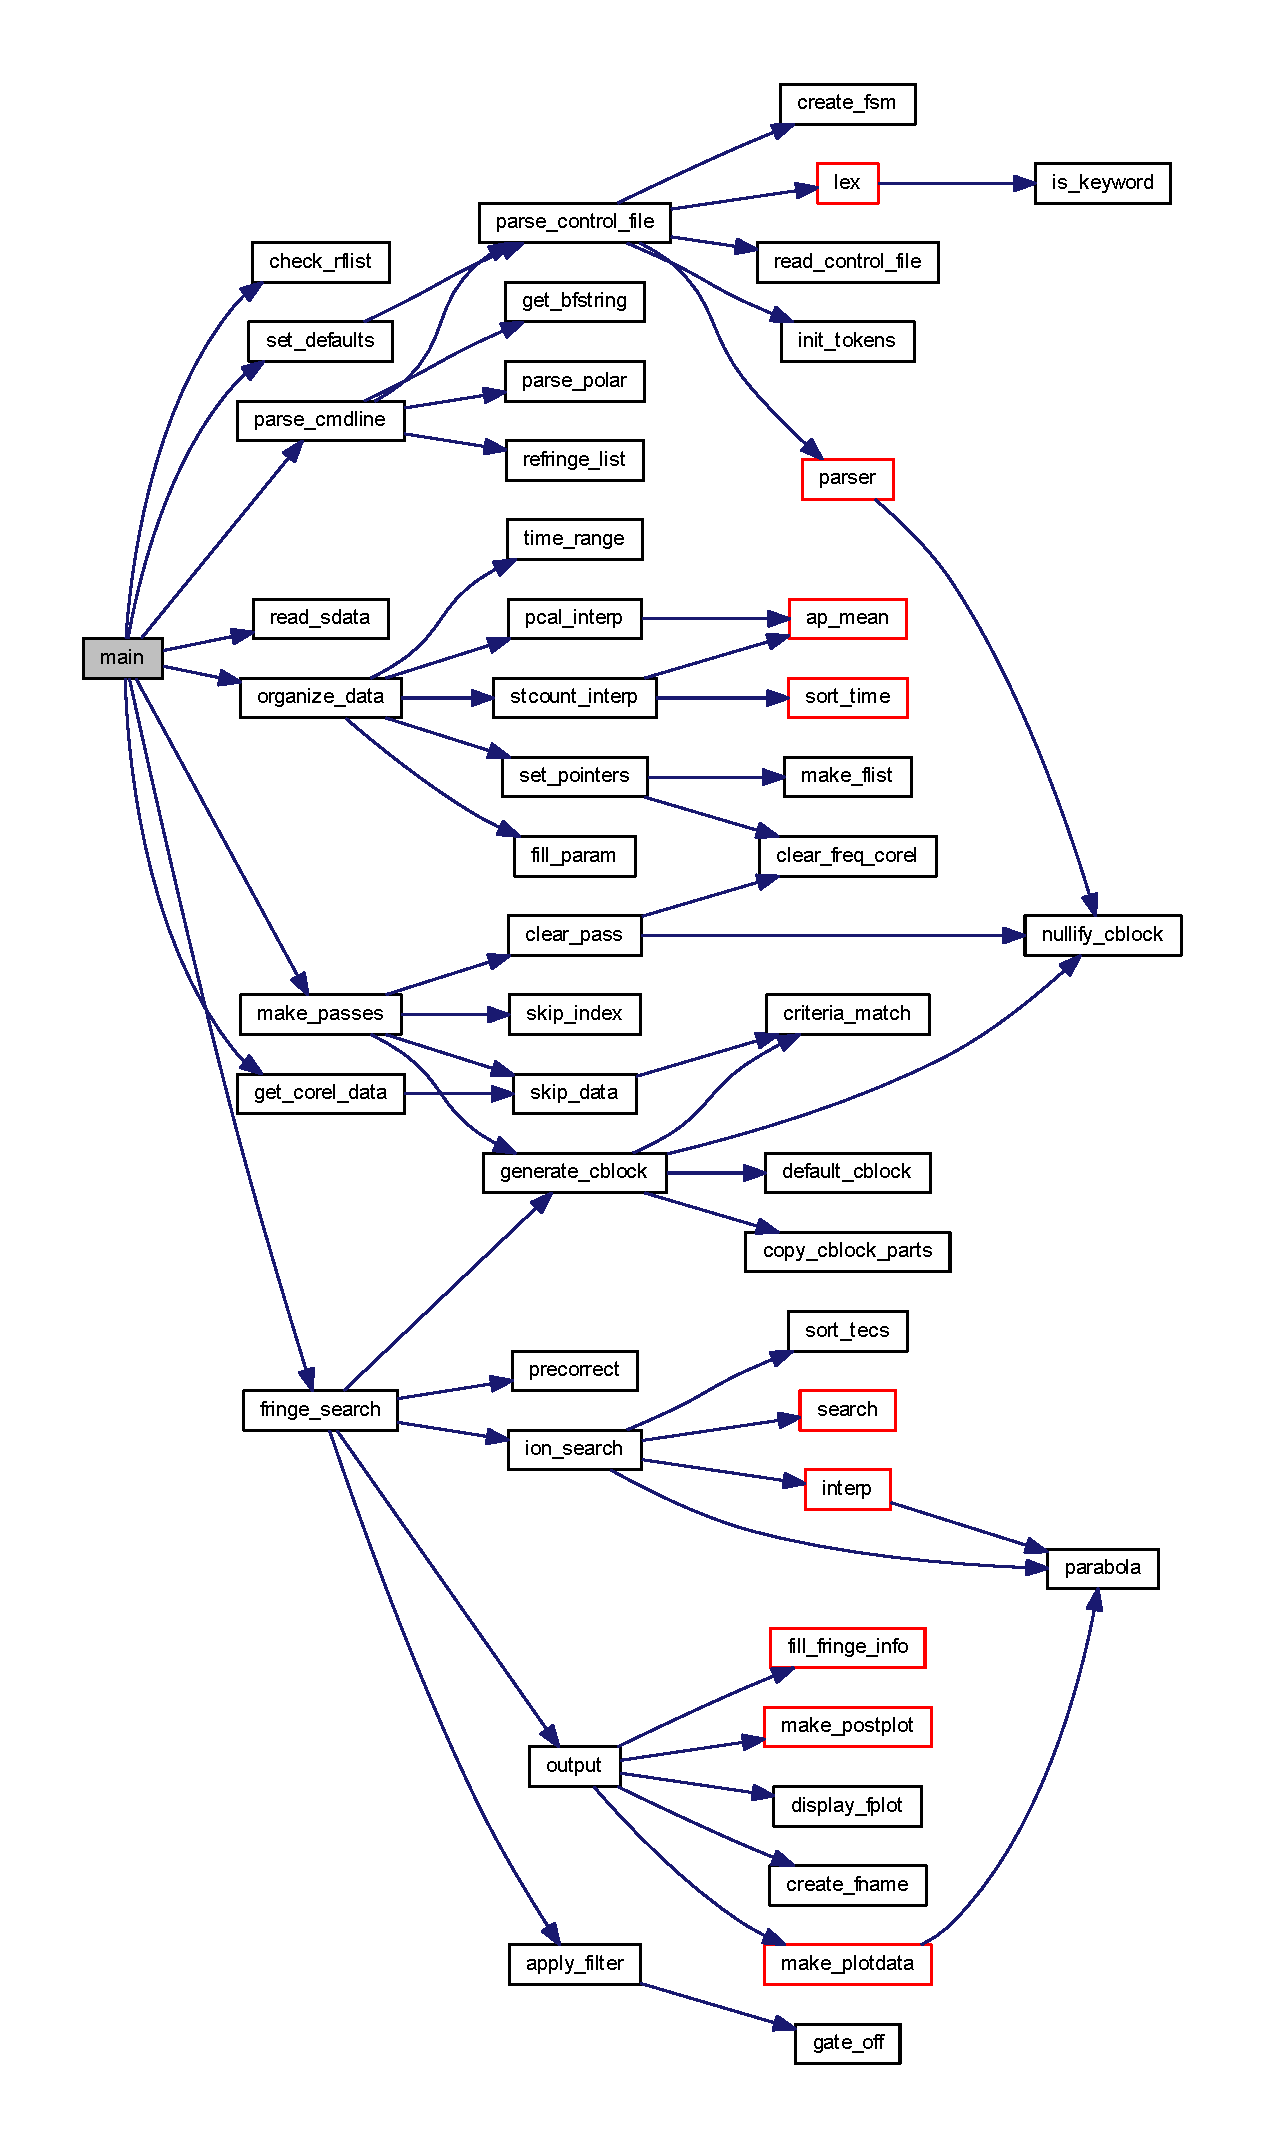
\includegraphics[width=.9\linewidth]{./fourfit_graph.pdf}
  \label{fig:fourfitgraph}
\end{figure}

\begin{figure}[tb]
  \centering
  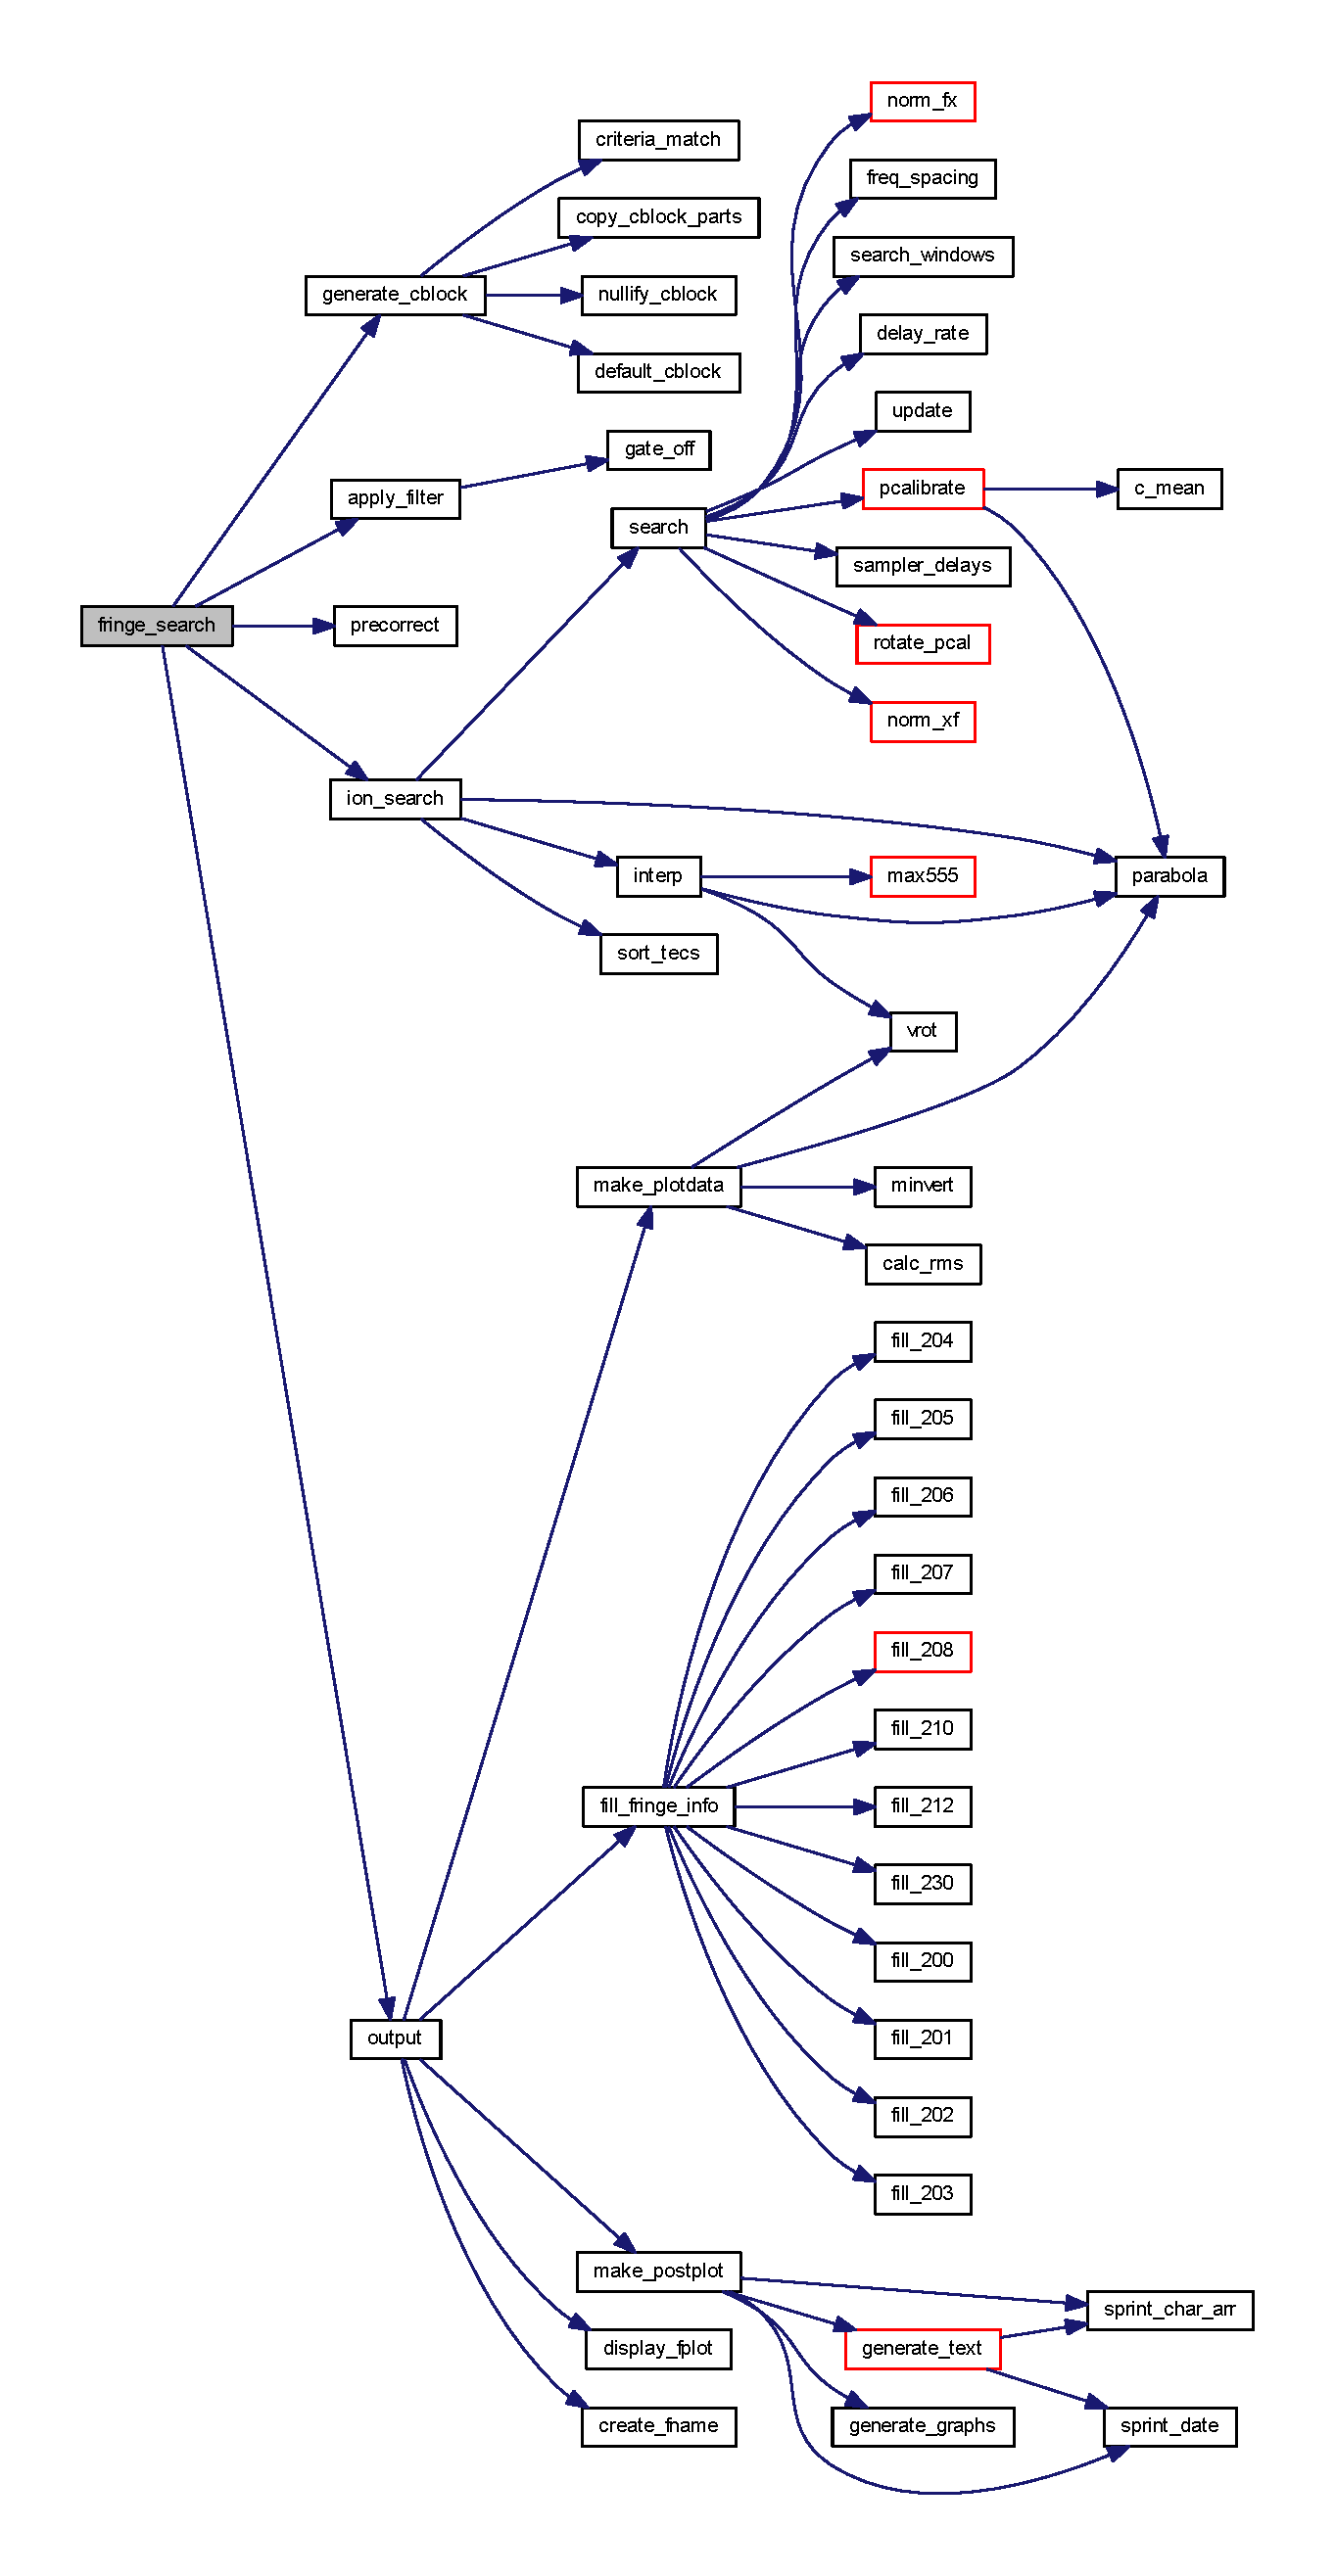
\includegraphics[width=.9\linewidth]{./fringe_search_graph.pdf}
  \label{fig:fringesearchgraph}
\end{figure}

\begin{figure}[tb]
  \centering
  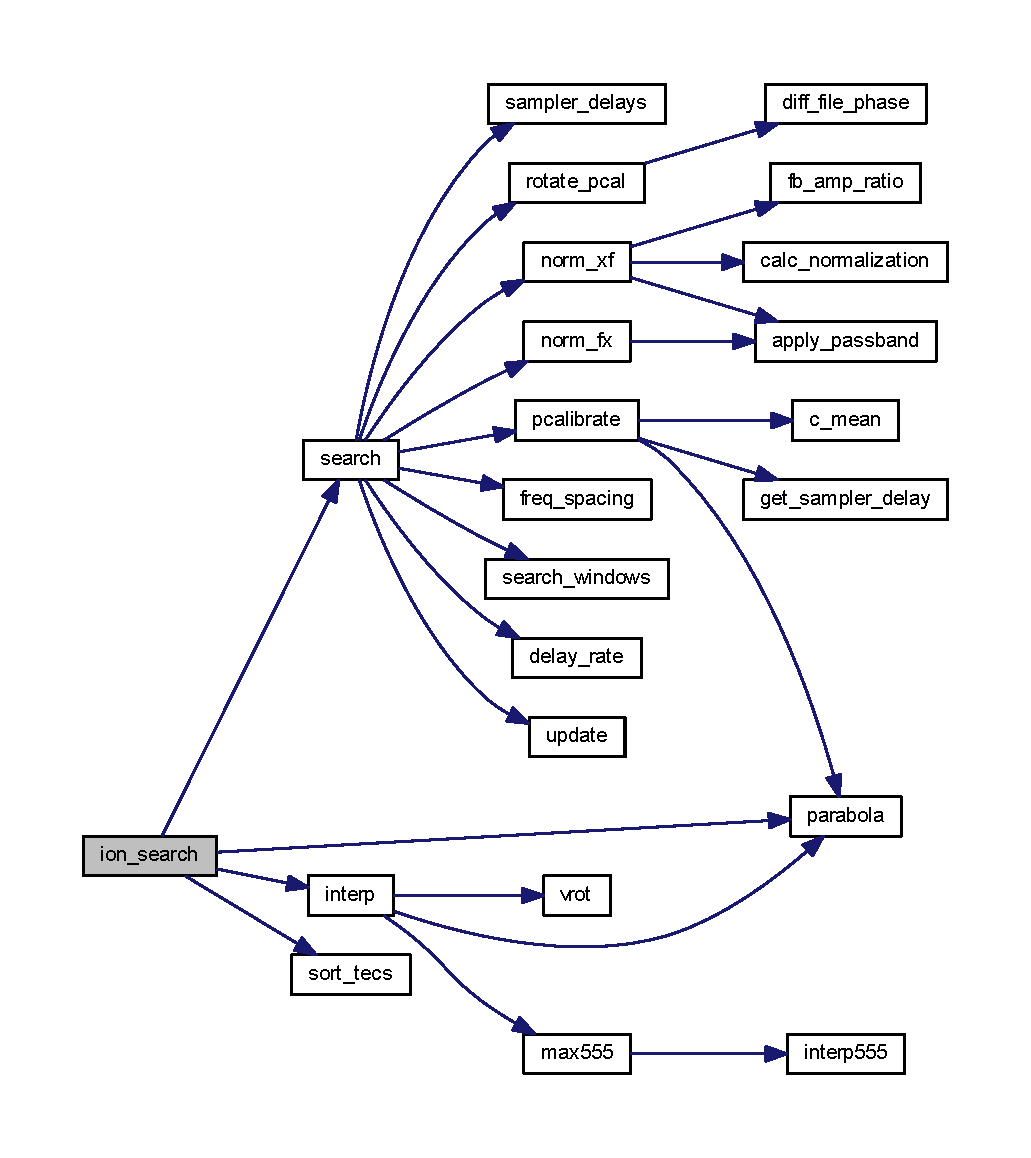
\includegraphics[width=.9\linewidth]{./ion_search_graph.pdf}
  \label{fig:ionsearchgraph}
\end{figure}

\begin{figure}[tb]
  \centering
  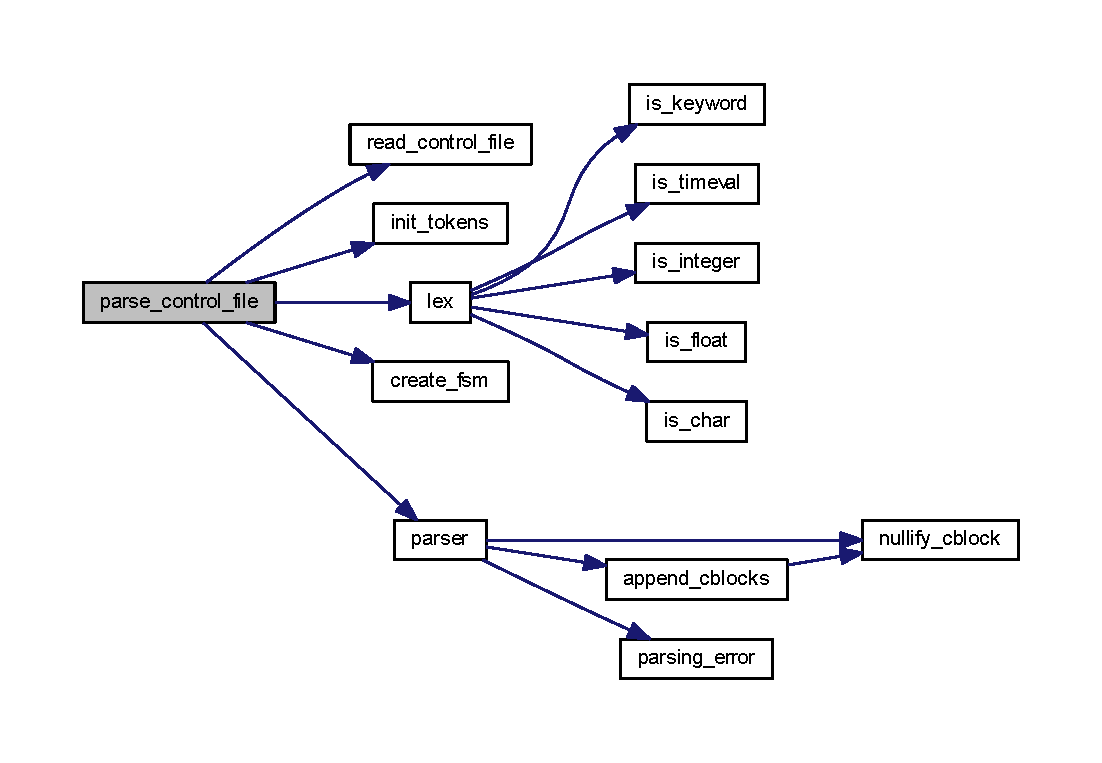
\includegraphics[width=.9\linewidth]{./parse_control_file_graph.pdf}
  \label{fig:parsecfgraph}
\end{figure}




\end{appendices}
\end{document}

